\chapter{Geometria}

Geometrisissä tehtävissä on usein haasteena keksiä,
mistä suunnasta ongelmaa kannattaa lähestyä,
jotta ratkaisun saa koodattua mukavasti ja
erikoistapauksia tulee mahdollisimman vähän.
Tässä luvussa tutustumme tekniikoihin, jotka helpottavat
geometristen algoritmien toteutusta.

\section{Kompleksiluvut}

Kompleksiluku on luku muotoa $x+y i$, missä $i = \sqrt{-1}$
on imaginääriyksikkö.
Kompleksiluvun luonteva geometrinen tulkinta on,
että se esittää kaksiulotteisen tason pistettä $(x,y)$
tai vektoria origosta pisteeseen $(x,y)$.

Esimerkiksi luku $4+2i$ tarkoittaa seuraavaa
pistettä ja vektoria:
\\
\begin{center}
\begin{tikzpicture}[scale=0.45]

\draw[->,thick] (-5,0)--(5,0);
\draw[->,thick] (0,-5)--(0,5);

\draw[fill] (4,2) circle [radius=0.1];
\draw[->,thick] (0,0)--(4-0.1,2-0.1);

\node at (4,2.8) {$(4,2)$};
\end{tikzpicture}
\end{center}

C++:ssa on kompleksilukujen käsittelyyn luokka \texttt{complex},
josta on hyötyä geometriassa,
koska sen avulla voi esittää pisteen tai vektorin
kompleksilukuna ja luokassa on valmiita
geometriaan soveltuvia työkaluja.

Seuraavassa koodissa \texttt{C} on koordinaatin tyyppi
ja \texttt{P} on pisteen tai vektorin tyyppi.
Lisäksi koodi määrittelee
lyhennysmerkinnät \texttt{X} ja \texttt{Y},
joiden avulla pystyy viittaamaan x- ja y-koordinaatteihin.

\begin{lstlisting}
typedef long long C;
typedef complex<C> P;
#define X real()
#define Y imag()
\end{lstlisting}

Esimerkiksi seuraava koodi määrittelee pisteen $p=(4,2)$
ja ilmoittaa sen x- ja y-koordinaatin:

\begin{lstlisting}
P p = {4,2};
cout << p.X << " " << p.Y << "\n"; // 4 2
\end{lstlisting}

Seuraava koodi määrittelee vektorit $v=(3,1)$
ja $u=(2,2)$ ja laskee sitten niiden summan $s=v+u$:

\begin{lstlisting}
P v = {3,1};
P u = {2,2};
P s = v+u;
cout << s.X << " " << s.Y << "\n"; // 5 3
\end{lstlisting}

Sopiva tyyppi koordinaatille on tilanteesta
riippuen \texttt{long long} (kokonaisluku)
tai \texttt{long double} (liukuluku).
Kokonaislukuja kannattaa käyttää aina kun mahdollista,
koska silloin laskenta on tarkkaa.

Jos koordinaatit ovat liukulukuja,
niiden vertailussa täytyy ottaa huomioon epätarkkuus.
Turvallinen tapa tarkistaa,
ovatko liukuluvut $a$ ja $b$ samat
on käyttää vertailua $|a-b|<\epsilon$, jossa $\epsilon$
on pieni luku (esimerkiksi $\epsilon=10^{-9}$).

\subsubsection*{Funktioita}

Seuraavissa esimerkeissä pisteen tyyppinä on
\texttt{long double}:

Funktio \texttt{abs(v)} laskee vektorin $v=(x,y)$
pituuden $|v|$ kaavalla $\sqrt{x^2+y^2}$.
Sillä voi laskea myös pisteiden $(x_1,y_1)$
ja $(x_2,y_2)$ etäisyyden,
koska pisteiden etäisyys
on sama kuin vektorin $(x_2-x_1,y_2-y_1)$ pituus.
Joskus hyödyllinen on myös funktio \texttt{norm(v)},
joka laskee vektorin $v=(x,y)$ pituuden neliön $|v|^2$.

Seuraava koodi laskee
pisteiden $(4,2)$ ja $(3,-1)$ etäisyyden:
\begin{lstlisting}
P a = {4,2};
P b = {3,-1};
cout << abs(b-a) << "\n"; // 3.60555
\end{lstlisting}

Funktio \texttt{arg(v)} laskee vektorin $v=(x,y)$
kulman radiaaneina suhteessa x-akseliin.
Radiaaneina ilmoitettu kulma $r$ vastaa asteina
kulmaa $180 \cdot r/\pi$ astetta.
Jos vektori osoittaa suoraan oikealle,
sen kulma on 0.
Kulma kasvaa vastapäivään ja vähenee myötäpäivään
liikuttaessa.

Funktio \texttt{polar(s,a)} muodostaa vektorin,
jonka pituus on $s$ ja joka osoittaa kulmaan $a$.
Lisäksi vektoria pystyy kääntämään kulman $a$
verran kertomalla se vektorilla,
jonka pituus on 1 ja kulma on $a$.

Seuraava koodi laskee vektorin $(4,2)$ kulman,
kääntää sitä sitten $1/2$ radiaania vastapäivään
ja laskee uuden kulman:

\begin{lstlisting}
P v = {4,2};
cout << arg(v) << "\n"; // 0.463648
v *= polar(1.0,0.5);
cout << arg(v) << "\n"; // 0.963648
\end{lstlisting}

\section{Pisteen sijainti}

\subsection{Ristitulo}

Vektorien
$a=(x_1,y_1)$ ja $b=(x_2,y_2)$ ristitulo $a \times b$
lasketaan kaavalla $x_1 y_2 - x_2 y_1$.
Ristitulo ilmaisee, mihin suuntaan vektori $b$
kääntyy, jos se laitetaan vektorin $a$ perään.
Positiivinen ristitulo tarkoittaa käännöstä vasemmalle,
negatiivinen käännöstä oikealle, ja nolla tarkoittaa,
että vektorit ovat samalla suoralla.

Seuraava kuva näyttää kolme esimerkkiä ristitulosta:
\\
\begin{center}
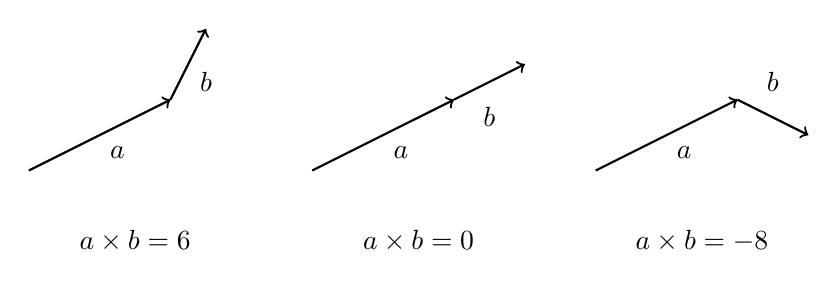
\begin{tikzpicture}[scale=0.45]

\draw[->,thick] (0,0)--(4,2);
\draw[->,thick] (4,2)--(4+1,2+2);

\node at (2.5,0.5) {$a$};
\node at (5,2.5) {$b$};

\node at (3,-2) {$a \times b = 6$};

\draw[->,thick] (8+0,0)--(8+4,2);
\draw[->,thick] (8+4,2)--(8+4+2,2+1);

\node at (8+2.5,0.5) {$a$};
\node at (8+5,1.5) {$b$};

\node at (8+3,-2) {$a \times b = 0$};

\draw[->,thick] (16+0,0)--(16+4,2);
\draw[->,thick] (16+4,2)--(16+4+2,2-1);

\node at (16+2.5,0.5) {$a$};
\node at (16+5,2.5) {$b$};

\node at (16+3,-2) {$a \times b = -8$};
\end{tikzpicture}
\end{center}

\noindent
Luokkaa \texttt{complex} käyttäen vektorien
$a$ ja $b$ ristitulon voi laskea näin:

\begin{lstlisting}
P a = {4,2};
P b = {1,2};
C r = (conj(a)*b).Y; // 6
\end{lstlisting}

Tämä perustuu siihen, että funktio \texttt{conj}
muuttaa vektorin y-koordinaatin käänteiseksi
ja kompleksilukujen kertolaskun seurauksena
vektorien $(x_1,-y_1)$ ja $(x_2,y_2)$
kertolaskun y-koordinaatti on $x_1 y_2 - x_2 y_1$.

\subsection{Suora ja piste}

Ristitulon avulla voi selvittää,
kummalla puolella suoraa tutkittava piste sijaitsee.
Oletetaan, että suora kulkee pisteiden
$s_1$ ja $s_2$ kautta, katsontasuunta on
pisteestä $s_1$ pisteeseen $s_2$ ja
tutkittava piste on $p$.

Esimerkiksi seuraavassa kuvassa piste $p$
on suoran vasemmalla puolella:
\\
\begin{center}
\begin{tikzpicture}[scale=0.45]
\draw[dashed,thick,->] (0,0)--(12,3);
\draw[fill] (4,1) circle [radius=0.1];
\draw[fill] (8,2) circle [radius=0.1];
\draw[fill] (5,3) circle [radius=0.1];
\node at (4,0) {$s_1$};
\node at (8,1) {$s_2$};
\node at (5,4) {$p$};
\end{tikzpicture}
\end{center}

Ristitulo $(p-s_1) \times (p-s_2)$
kertoo, kummalla puolella suoraa piste sijaitsee.
Jos ristitulo on positiivinen,
piste $p$ on suoran vasemmalla puolella,
ja jos ristitulo on negatiivinen,
piste $p$ on suoran oikealla puolella.
Jos taas ristitulo on nolla,
piste $p$ on pisteiden $s_1$ ja $s_2$
kanssa suoralla.

\subsection{Janojen leikkaus}

Usein esiintyvä tehtävä on selvittää,
leikkaavatko kaksi janaa.
Esimerkiksi seuraavassa kuvassa
janat $ab$ ja $cd$ leikkaavat pisteessä $p$.
\\
\begin{center}
\begin{tikzpicture}[scale=0.9]
\draw (0,1)--(6,3);
\draw (2,4)--(4,0);
\draw[fill] (0,1) circle [radius=0.05];
\node at (0,0.5) {$c$};
\draw[fill] (6,3) circle [radius=0.05];
\node at (6,2.5) {$d$};
\draw[fill] (2,4) circle [radius=0.05];
\node at (1.5,3.5) {$a$};
\draw[fill] (4,0) circle [radius=0.05];
\node at (4,-0.4) {$b$};
\draw[fill] (3,2) circle [radius=0.05];
\node at (3,1.5) {$p$};
\end{tikzpicture}
\end{center}

Oletetaan, että janat eivät ole samalla suoralla
eikä niillä ole yhteisiä päätepisteitä.
Tässä tapauksessa janat leikkaavat
tarkalleen silloin, kun samaan aikaan
pisteet $c$ ja $d$ ovat eri puolilla
$a$:sta $b$:hen kulkevaa suoraa
ja pisteet $a$ ja $b$
ovat eri puolilla 
$c$:stä $d$:hen kulkevaa suoraa.

Janojen leikkauspiste $p$ selviää etsimällä
parametrit $t$ ja $u$ niin, että

\[ p = a+t(b-a) = c+u(d-c). \]

\subsection{Piste monikulmiossa}

Kätevä keino tarkistaa,
onko piste monikulmion sisällä,
on lähettää pisteestä säde
satunnaiseen suuntaan ja laskea,
montako kertaa se osuu monikulmion reunaan.
Jos kertoja on pariton määrä,
piste on sisäpuolella,
ja jos kertoja on parillinen määrä,
piste on ulkopuolella.
% 
% Annettuna on monikulmio ja piste,
% ja tehtävänä on selvittää,
% onko piste monikulmion sisäpuolella vai ulkopuolella.
% Esimerkiksi seuraavassa kuvassa
% piste $a$ on monikulmion sisäpuolella,
% kun taas piste $b$ on ulkopuolella.
% \\
% \begin{center}
% \begin{tikzpicture}[scale=0.7]
% \draw (0,0)--(2,-2)--(3,1)--(5,1)--(2,3)--(1,2)--(-1,2)--(1,4)--(-2,4)--(-2,1)--(-3,3)--(-4,0)--(0,0);
% 
% \draw[fill] (-3,1) circle [radius=0.05];
% \node at (-3,0.5) {$a$};
% \draw[fill] (1,3) circle [radius=0.05];
% \node at (1,2.5) {$b$};
% \end{tikzpicture}
% \end{center}
% 
% 
% \newpage

Esimerkiksi seuraavassa kuvassa piste $a$ on monikulmion
sisäpuolella ja piste $b$ on ulkopuolella.
Kuvassa on myös joitakin pisteistä lähteviä säteitä.
\\
\begin{center}
\begin{tikzpicture}[scale=0.75]
\draw (0,0)--(2,-2)--(3,1)--(5,1)--(2,3)--(1,2)--(-1,2)--(1,4)--(-2,4)--(-2,1)--(-3,3)--(-4,0)--(0,0);

\draw[fill] (-3,1) circle [radius=0.05];
\node at (-3,0.5) {$a$};
\draw[fill] (1,3) circle [radius=0.05];
\node at (1,2.5) {$b$};

\draw[dashed,->] (-3,1)--(-6,0);
\draw[dashed,->] (-3,1)--(0,5);

\draw[dashed,->] (1,3)--(4,-1);
\draw[dashed,->] (1,3)--(3,4);
\end{tikzpicture}
\end{center}

Pisteestä $a$ lähtevät säteet osuvat 1 ja 3
kertaa monikulmion reunaan,
joten piste on sisäpuolella.
Vastaavasti pisteestä $b$ lähtevät
säteet osuvat 0 ja 2 kertaa monikulmion reunaan,
joten piste on ulkopuolella.

\section{Pinta-alat}

\subsection{Kolmion pinta-ala}

Kolmion pinta-alan laskemiseen on monia tapoja.
Koulusta tuttu kaava on

\[\frac{bh}{2},\]

\noindent
missä $b$ on kannan pituus ja $h$ on korkeus.

Heronin kaava

\[ \sqrt{s (s-a) (s-b) (s-c)} \]

\noindent
laskee pinta-alan, kun sivujen pituudet ovat
$a$, $b$ ja $c$, ja $s=(a+b+c)/2$.

Pinta-alan voi laskea myös ristitulon avulla
kaavalla

\[ \frac{1}{2} ((p_2-p_1) \times (p_3-p_1)), \]

\noindent
missä kolmion kärkipisteet ovat $p_1=(x_1,y_1)$,
$p_2=(x_2,y_2)$ ja $p_3=(x_3,y_3)$.

\subsubsection*{Pisteen etäisyys suorasta}

Kolmion pinta-alan avulla voi selvittää,
kuinka kaukana piste on suorasta.
Esimerkiksi seuraavassa kuvassa $d$
on lyhin etäisyys pisteestä $p$ suoralle,
jonka määrittävät pisteet $s_1$ ja $s_2$:
\\
\begin{center}
\begin{tikzpicture}[scale=0.75]
\draw (-2,-1)--(6,3);
\draw[dashed] (1,4)--(2.40,1.2);
\node at (0,-0.5) {$s_1$};
\node at (4,1.5) {$s_2$};
\node at (0.5,4) {$p$};
\node at (2,2.7) {$d$};
\draw[fill] (0,0) circle [radius=0.05];
\draw[fill] (4,2) circle [radius=0.05];
\draw[fill] (1,4) circle [radius=0.05];
\end{tikzpicture}
\end{center}

Pisteiden $s_1$, $s_2$ ja $p$ muodostaman kolmion
pinta-ala on toisaalta $\frac{1}{2} |s_2-s_1| d$ ja toisaalta
$\frac{1}{2} ((s_1-p) \times (s_2-p))$,
joten etäisyys on

\[ d = \frac{(s_1-p) \times (s_2-p)}{|s_2-s_1|} .\]


\subsection{Monikulmion pinta-ala}

Yleinen kaava monikulmion pinta-alan laskemiseen on

\[\frac{1}{2} |\sum_{i=1}^{i=n-1} (p_i \times p_{i+1})|, \]

missä monikulmion kärkipisteet ovat
järjestyksessä $p_1,p_2,\ldots,p_n$
ja ensimmäinen ja viimeinen kärkipiste
ovat samat eli $p_1=p_n$.

Esimerkiksi monikulmion
\begin{center}
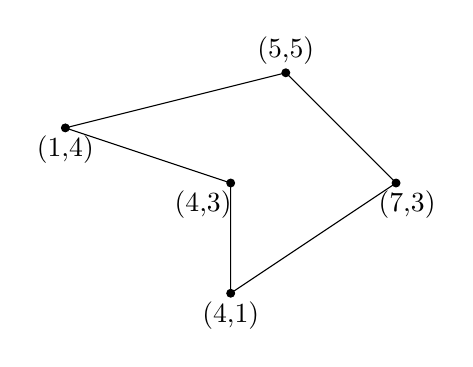
\begin{tikzpicture}[scale=0.7]
\filldraw (4,1.4) circle (2pt);
\filldraw (7,3.4) circle (2pt);
\filldraw (5,5.4) circle (2pt);
\filldraw (1,4.4) circle (2pt);
\filldraw (4,3.4) circle (2pt);
\node (1) at (4,1) {(4,1)};
\node (2) at (7.2,3) {(7,3)};
\node (3) at (5,5.8) {(5,5)};
\node (4) at (1,4) {(1,4)};
\node (5) at (3.5,3) {(4,3)};
\path[draw] (4,1.4) -- (7,3.4) -- (5,5.4) -- (1,4.4) -- (4,3.4) -- (4,1.4);
\end{tikzpicture}
\end{center}

pinta-ala on

\[\frac{|(4\cdot3-7\cdot1)+(7\cdot5-5\cdot3)+(5\cdot4-1\cdot5)+(1\cdot3-4\cdot4)+(4\cdot1-4\cdot3)|}{2} = 19/2.\]

\subsection{Pickin lause}

Toinen tapa laskea monikulmion pinta-ala
on käyttää Pickin lausetta.
Se pätee silloin, kun kaikki kärkipisteet ovat
kokonaislukupisteissä.
Pickin lauseen mukaan monikulmion pinta-ala on

\[ a + b/2 -1, \]

missä $a$ on kokonaislukupisteiden määrä monikulmion sisällä
ja $b$ on kokonaislukupisteiden määrä monikulmion reunalla.

Esimerkiksi monikulmion
\begin{center}
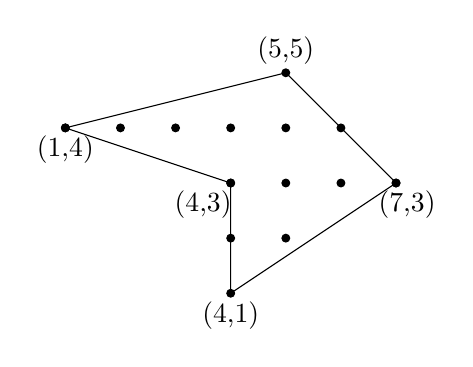
\begin{tikzpicture}[scale=0.7]
\filldraw (4,1.4) circle (2pt);
\filldraw (7,3.4) circle (2pt);
\filldraw (5,5.4) circle (2pt);
\filldraw (1,4.4) circle (2pt);
\filldraw (4,3.4) circle (2pt);
\node (1) at (4,1) {(4,1)};
\node (2) at (7.2,3) {(7,3)};
\node (3) at (5,5.8) {(5,5)};
\node (4) at (1,4) {(1,4)};
\node (5) at (3.5,3) {(4,3)};
\path[draw] (4,1.4) -- (7,3.4) -- (5,5.4) -- (1,4.4) -- (4,3.4) -- (4,1.4);

\filldraw (1,4.4) circle (2pt);
\filldraw (2,4.4) circle (2pt);
\filldraw (3,4.4) circle (2pt);
\filldraw (4,4.4) circle (2pt);
\filldraw (5,4.4) circle (2pt);
\filldraw (6,4.4) circle (2pt);

\filldraw (4,3.4) circle (2pt);
\filldraw (5,3.4) circle (2pt);
\filldraw (6,3.4) circle (2pt);
\filldraw (7,3.4) circle (2pt);

\filldraw (4,2.4) circle (2pt);
\filldraw (5,2.4) circle (2pt);
\end{tikzpicture}
\end{center}

pinta-ala on $7+7/2-1=19/2$.

